\documentclass[
10pt, % Set the default font size, options include: 8pt, 9pt, 10pt, 11pt, 12pt, 14pt, 17pt, 20pt
%t, % Uncomment to vertically align all slide content to the top of the slide, rather than the default centered
aspectratio=169, % Uncomment to set the aspect ratio to a 16:9 ratio which matches the aspect ratio of 1080p and 4K screens and projectors
]{beamer}

\usepackage[all]{xy}

\usepackage[spanish]{babel}
\usepackage[utf8]{inputenc}

\graphicspath{{Images/}{./}} % Specifies where to look for included images (trailing slash required)

\usepackage{booktabs} % Allows the use of \toprule, \midrule and \bottomrule for better rules in tables

%\usepackage{tikz}
%\usetikzlibrary{positioning}
%\usetikzlibrary{shapes,arrows,arrows,positioning,fit}

\usepackage{tikz}
\usetikzlibrary{mindmap}
\usetikzlibrary{arrows, positioning}
\usetikzlibrary{arrows, shapes, positioning, shadows, trees}

\usepackage{forest}

\usepackage{multirow}

\usepackage{graphicx, animate}
\usepackage{hyperref}

\usepackage{xcolor,listings}
\usepackage{textcomp}
%\usepackage{color}

\usepackage{enumitem}

\usepackage{xcolor}

\usepackage{verbatim}
\usepackage{changepage}

\usepackage{xmpmulti}

\providecommand{\abs}[1]{\lvert#1\rvert}

%----------------------------------------------------------------------------------------
%	SELECT LAYOUT THEME
%----------------------------------------------------------------------------------------
\usetheme{Madrid} 

%----------------------------------------------------------------------------------------
%	SELECT COLOR THEME
%----------------------------------------------------------------------------------------
%\usecolortheme{beaver}
%\usecolortheme{seahorse}
\usecolortheme{spruce} % verde suave
%\usecolortheme{whale}
%\usecolortheme{wolverine}

%----------------------------------------------------------------------------------------
%	SELECT FONT THEME & FONTS
%----------------------------------------------------------------------------------------
\usefonttheme{default} % Typeset using the default sans serif font
%\usefonttheme{serif} % Typeset using the default serif font (make sure a sans font isn't being set as the default font if you use this option!)
%\usefonttheme{structurebold} % Typeset important structure text (titles, headlines, footlines, sidebar, etc) in bold
%\usefonttheme{structureitalicserif} % Typeset important structure text (titles, headlines, footlines, sidebar, etc) in italic serif
%\usefonttheme{structuresmallcapsserif} % Typeset important structure text (titles, headlines, footlines, sidebar, etc) in small caps serif

%------------------------------------------------

%\usepackage{mathptmx} % Use the Times font for serif text
%\usepackage{palatino} % Use the Palatino font for serif text

\usepackage{helvet} % Use the Helvetica font for sans serif text
%\usepackage[default]{opensans} % Use the Open Sans font for sans serif text
%\usepackage[default]{FiraSans} % Use the Fira Sans font for sans serif text
\usepackage[default]{lato} % Use the Lato font for sans serif text

%----------------------------------------------------------------------------------------
%	SELECT INNER THEME
%----------------------------------------------------------------------------------------
\useinnertheme{circles}


\setbeamertemplate{footline} % Uncomment this line to remove the footer line in all slides
%\setbeamertemplate{footline}[page number] % Uncomment this line to replace the footer line in all slides with a simple slide count

\setbeamertemplate{navigation symbols}{} % Uncomment this line to remove the navigation symbols from the bottom of all slides

%----------------------------------------------------------------------------------------
%	PRESENTATION INFORMATION
%----------------------------------------------------------------------------------------

\title[Short Title]{Acercamiento al Procesamiento del Lenguaje Natural} 

\subtitle{Sistemas de Recuperación de Información}

\author{Lic. Carlos León González \\ Dra.C. Lucina García Hernández}

\institute[UC]{Facultad de Matem\'atica y Computaci\'on \\ Universidad de La Habana \\ \smallskip }

\date{29 de enero de  2024} % Presentation date or conference/meeting name, the optional parameter can contain a shortened version to appear on the bottom of every slide, while the required parameter value is output to the title slide

%----------------------------------------------------------------------------------------

\begin{document}
	
	\lstset{
		literate=%
		{á}{{\'a}}1
		{í}{{\'i}}1
		{é}{{\'e}}1
		{ý}{{\'y}}1
		{ú}{{\'u}}1
		{ó}{{\'o}}1
		{ě}{{\v{e}}}1
		{š}{{\v{s}}}1
		{č}{{\v{c}}}1
		{ř}{{\v{r}}}1
		{ž}{{\v{z}}}1
		{ď}{{\v{d}}}1
		{ť}{{\v{t}}}1
		{ň}{{\v{n}}}1                
		{ů}{{\r{u}}}1
		{Á}{{\'A}}1
		{Í}{{\'I}}1
		{É}{{\'E}}1
		{Ý}{{\'Y}}1
		{Ú}{{\'U}}1
		{Ó}{{\'O}}1
		{Ě}{{\v{E}}}1
		{Š}{{\v{S}}}1
		{Č}{{\v{C}}}1
		{Ř}{{\v{R}}}1
		{Ž}{{\v{Z}}}1
		{Ď}{{\v{D}}}1
		{Ť}{{\v{T}}}1
		{Ň}{{\v{N}}}1                
		{Ů}{{\r{U}}}1    
	}
	
	
	\begin{frame}
		\titlepage
	\end{frame}
	
	%------------------------------------------------
	% Motivación
	
	\begin{frame}
		
		\frametitle{¿Procesar texto influye en la recuperación?}
		
		\centering
		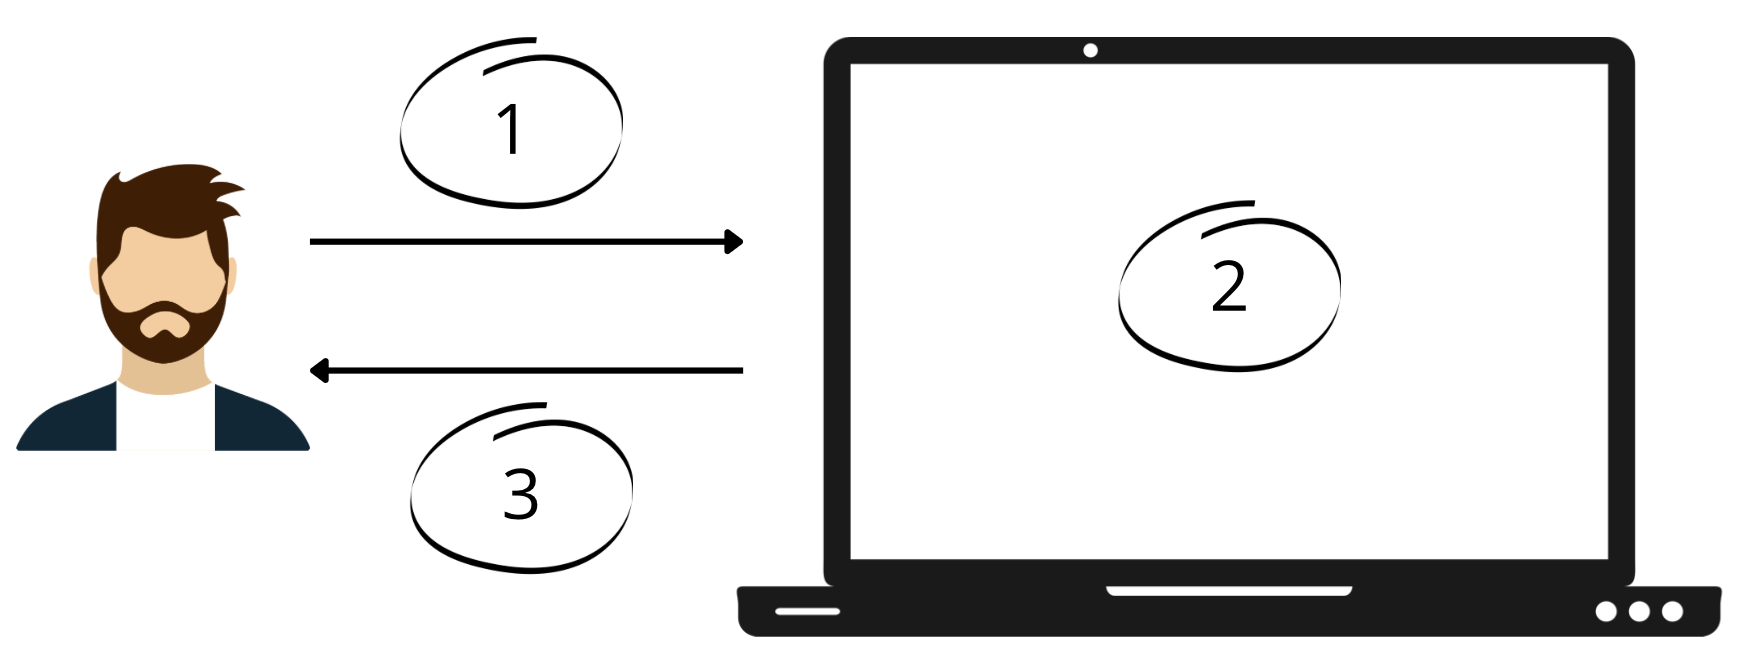
\includegraphics[scale=0.3]{motivacion.png} 
		
		%	\vspace{1\baselineskip}
		
		\begin{enumerate}
			
			\pause
			\item Consulta del usuario: \textbf{Necesito información sobre cómo cultivar plantas de rosa mosqueta}
			
			\vspace{1\baselineskip}
			\pause 
			\item Consulta procesada por el sistema: \textbf{Información sobre cultivar plantas de rosa mosqueta} \\ 
			
			\pause
			\vspace{1\baselineskip}
			El sistema reconocerá que:
			
			\begin{itemize}
				\item \textcolor{purple}{¿``cultivar'' y ``cultivo'' son conceptos similares?}
				
				\pause
				\item \textcolor{purple}{¿``rosa mosqueta'' y ``escaramujo'' referencian a la misma planta?}
				
				\pause
				\item \textcolor{purple}{¿``cultivar'' y ``cuidar'' son semáticamente similares en el contexto de las plantas?}
				
				\pause
				\item \textcolor{purple}{¿``rosa mosquite'' y ``rosa mosquete'' es la misma planta, a pesar del error ortográfico?}
			\end{itemize}
			
		\end{enumerate}
		
	\end{frame}
	
	%------------------------------------------------
	%
	
	\begin{frame}
		
		\frametitle{Procesamiento del Lenguaje Natural}
		
		\centering
		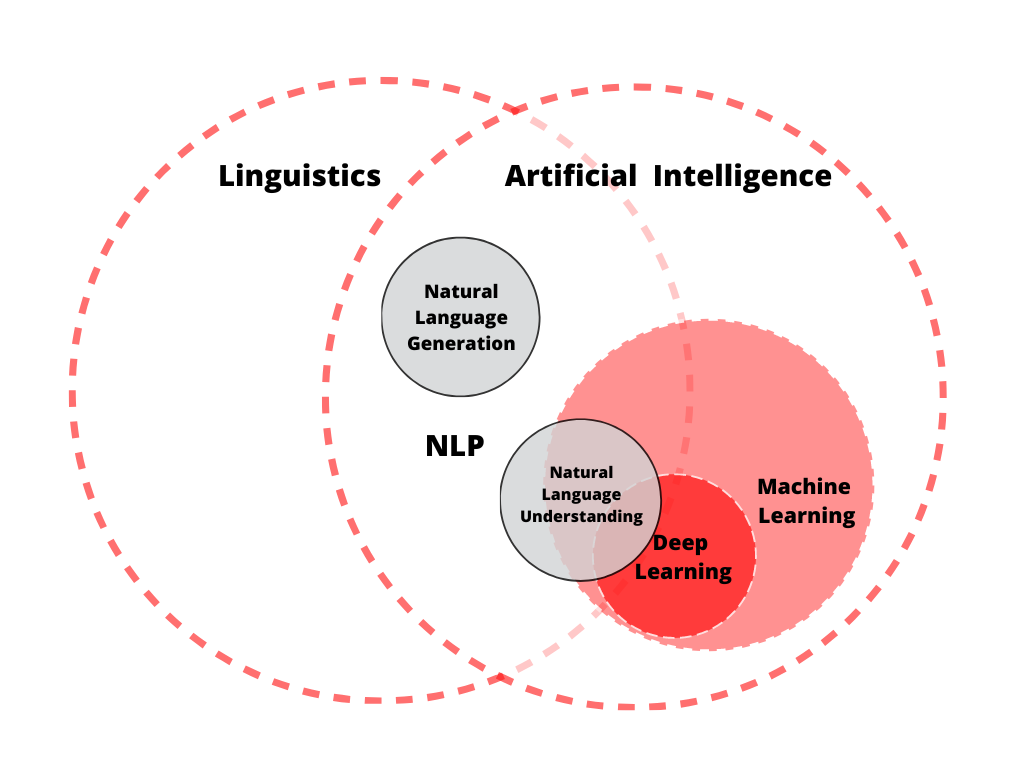
\includegraphics[scale=0.37]{Diagrama-IA.png} 
		
		%\vspace{3\baselineskip}
		{\scriptsize Tomado de \url{https://imbee.me/chatbots-nlp-que-son-y-para-que-sirven/}}
	
	\end{frame}
	
	
	%------------------------------------------------
	% Tokenización y Segmentación
	
	\begin{frame}
		
		\frametitle{Flujo de trabajo para el pre-procesamiento de un texto}
		
		% Explicación breve de cada una 
		
		\centering
		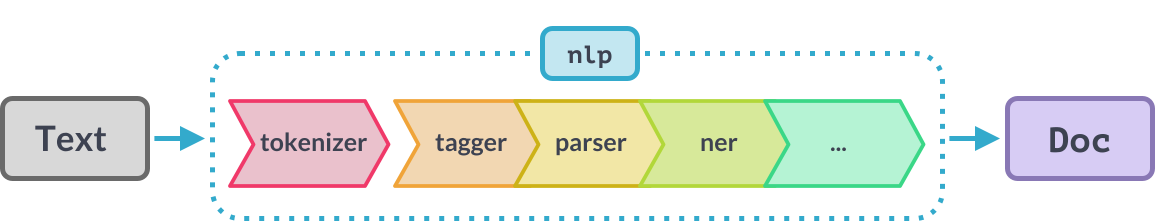
\includegraphics[scale=0.35]{pipeline.png} 
		
		\vspace{3\baselineskip}
		{\scriptsize Tomado de \url{https://spacy.io/usage/processing-pipelines}}
		
	\end{frame}
	
	%------------------------------------------------
	% Tokenizador 
	
	\begin{frame}
		
		\frametitle{Tokenizador}
		
		% \vspace{1\baselineskip}
		\begin{alertblock}{} 
			Objetivo: Encontrar los tokens (unidad lógica del vocabulario) dentro de cada texto. 
		\end{alertblock}
		
		\centering
		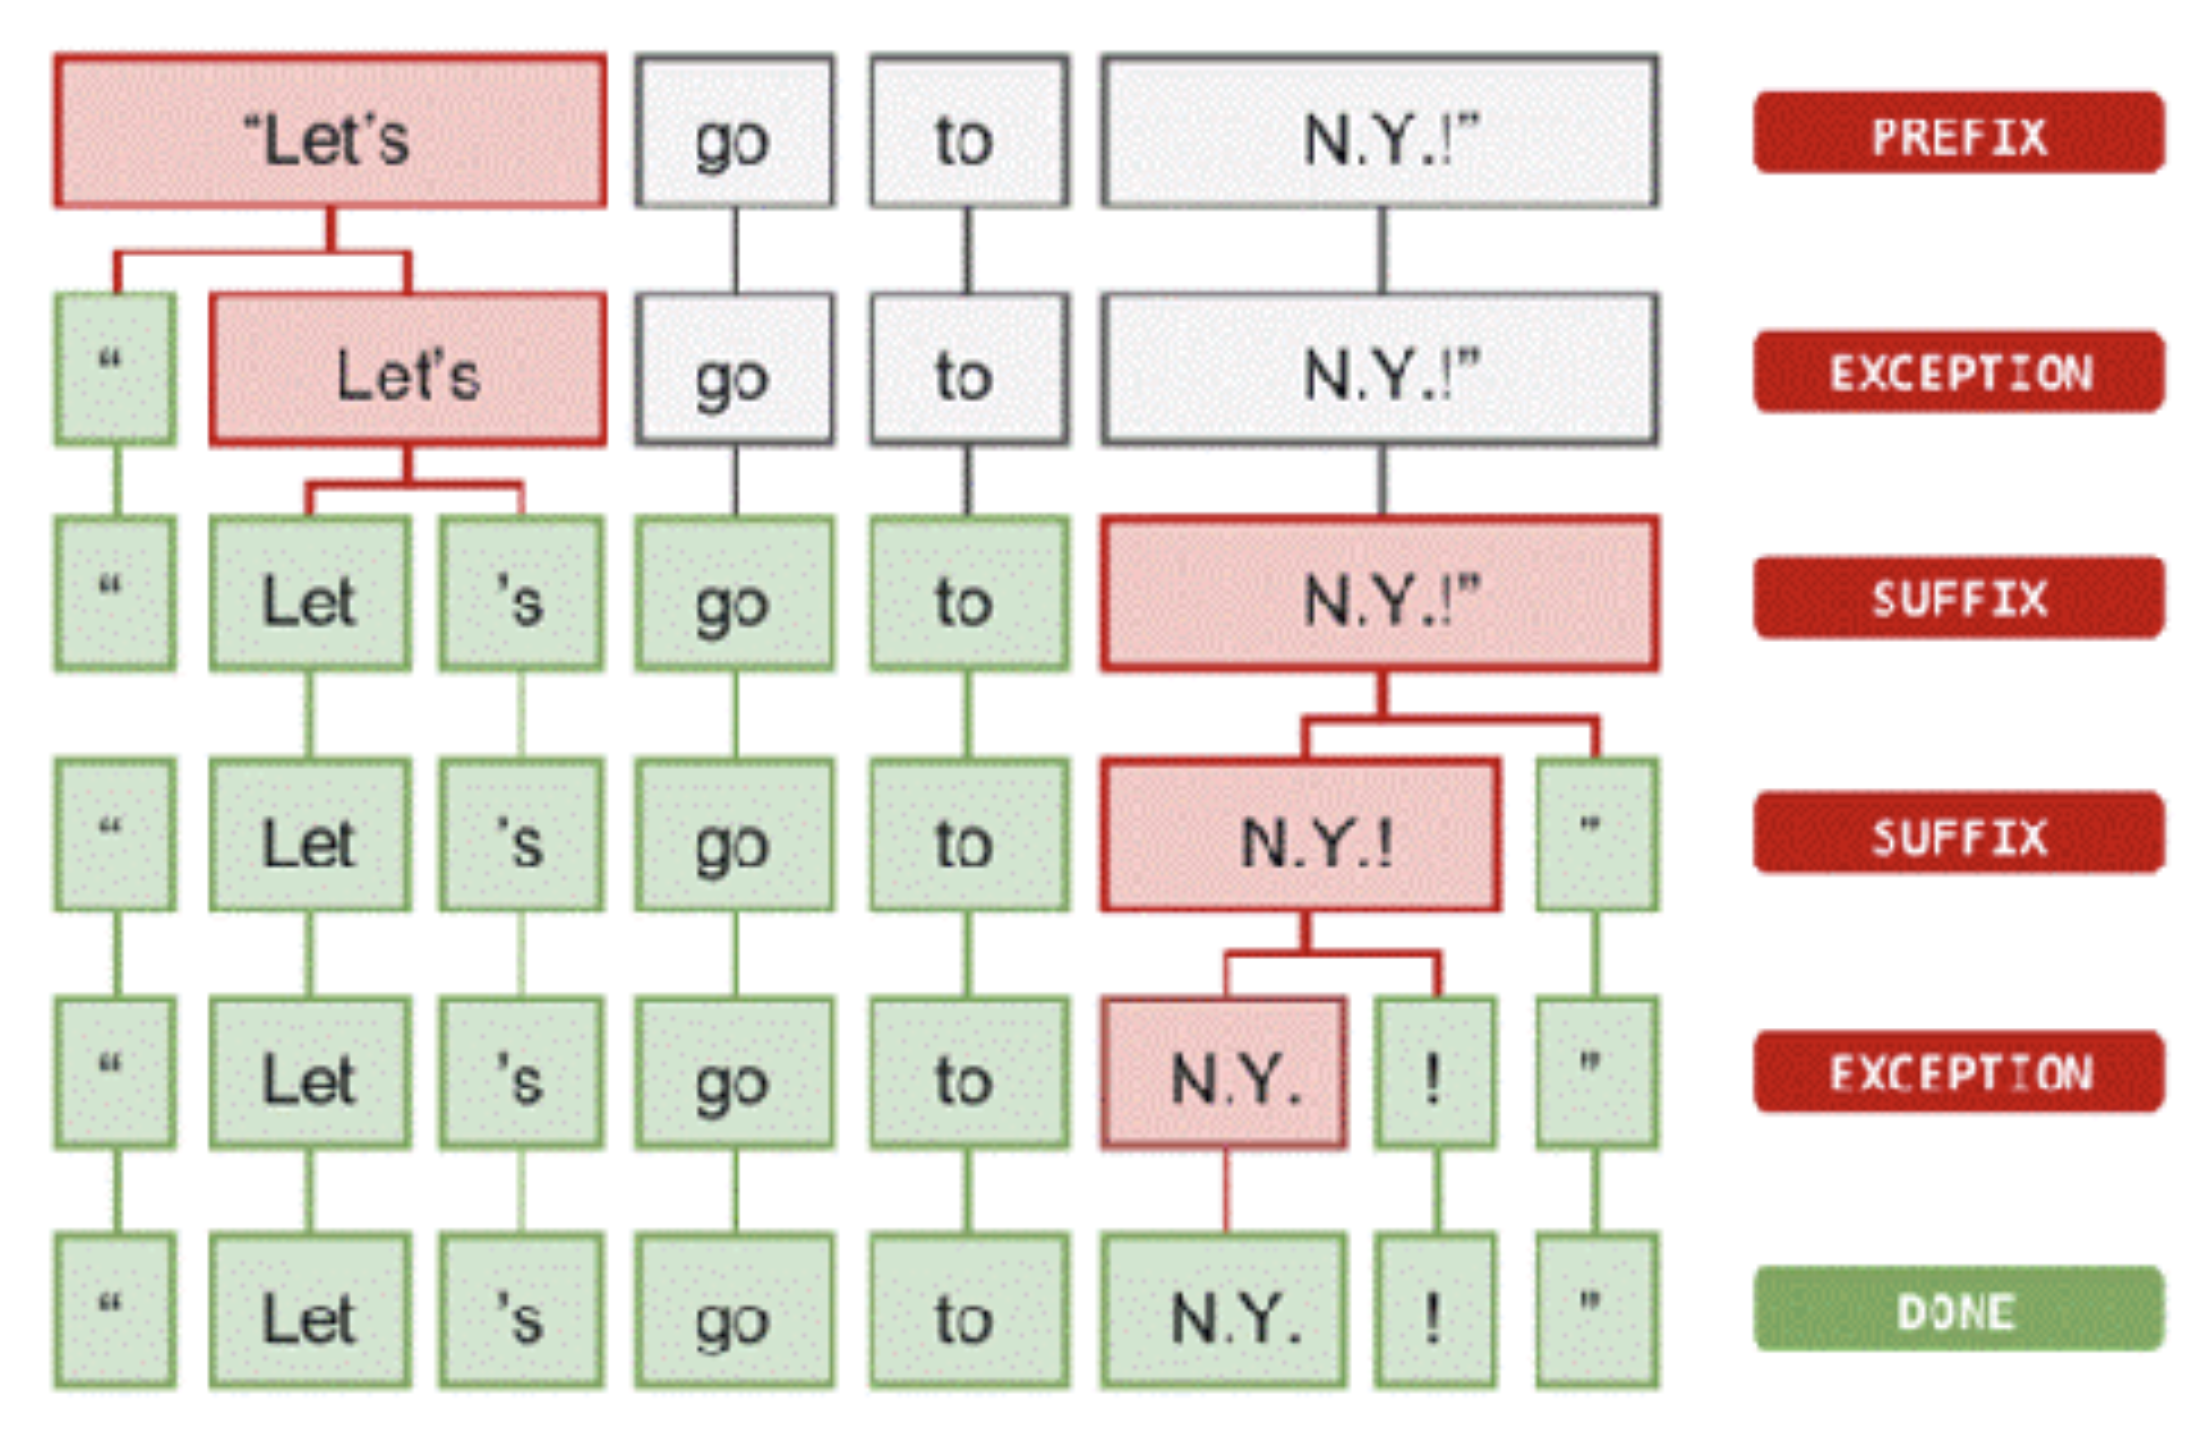
\includegraphics[scale=0.23]{tokenizador.png} 
		
		{\scriptsize Tomado de ``Srinivasa-Desikan, Bhargav, A practical guide to text analysis with Python, Gensim, spaCy, and Keras''.}
		
	\end{frame}
	
	%------------------------------------------------
	% Tipo de Tokenizador
	
	\begin{frame}
		
		\frametitle{Tipos de tokenizadores. Ventajas y desventajas}
		
		\centering
		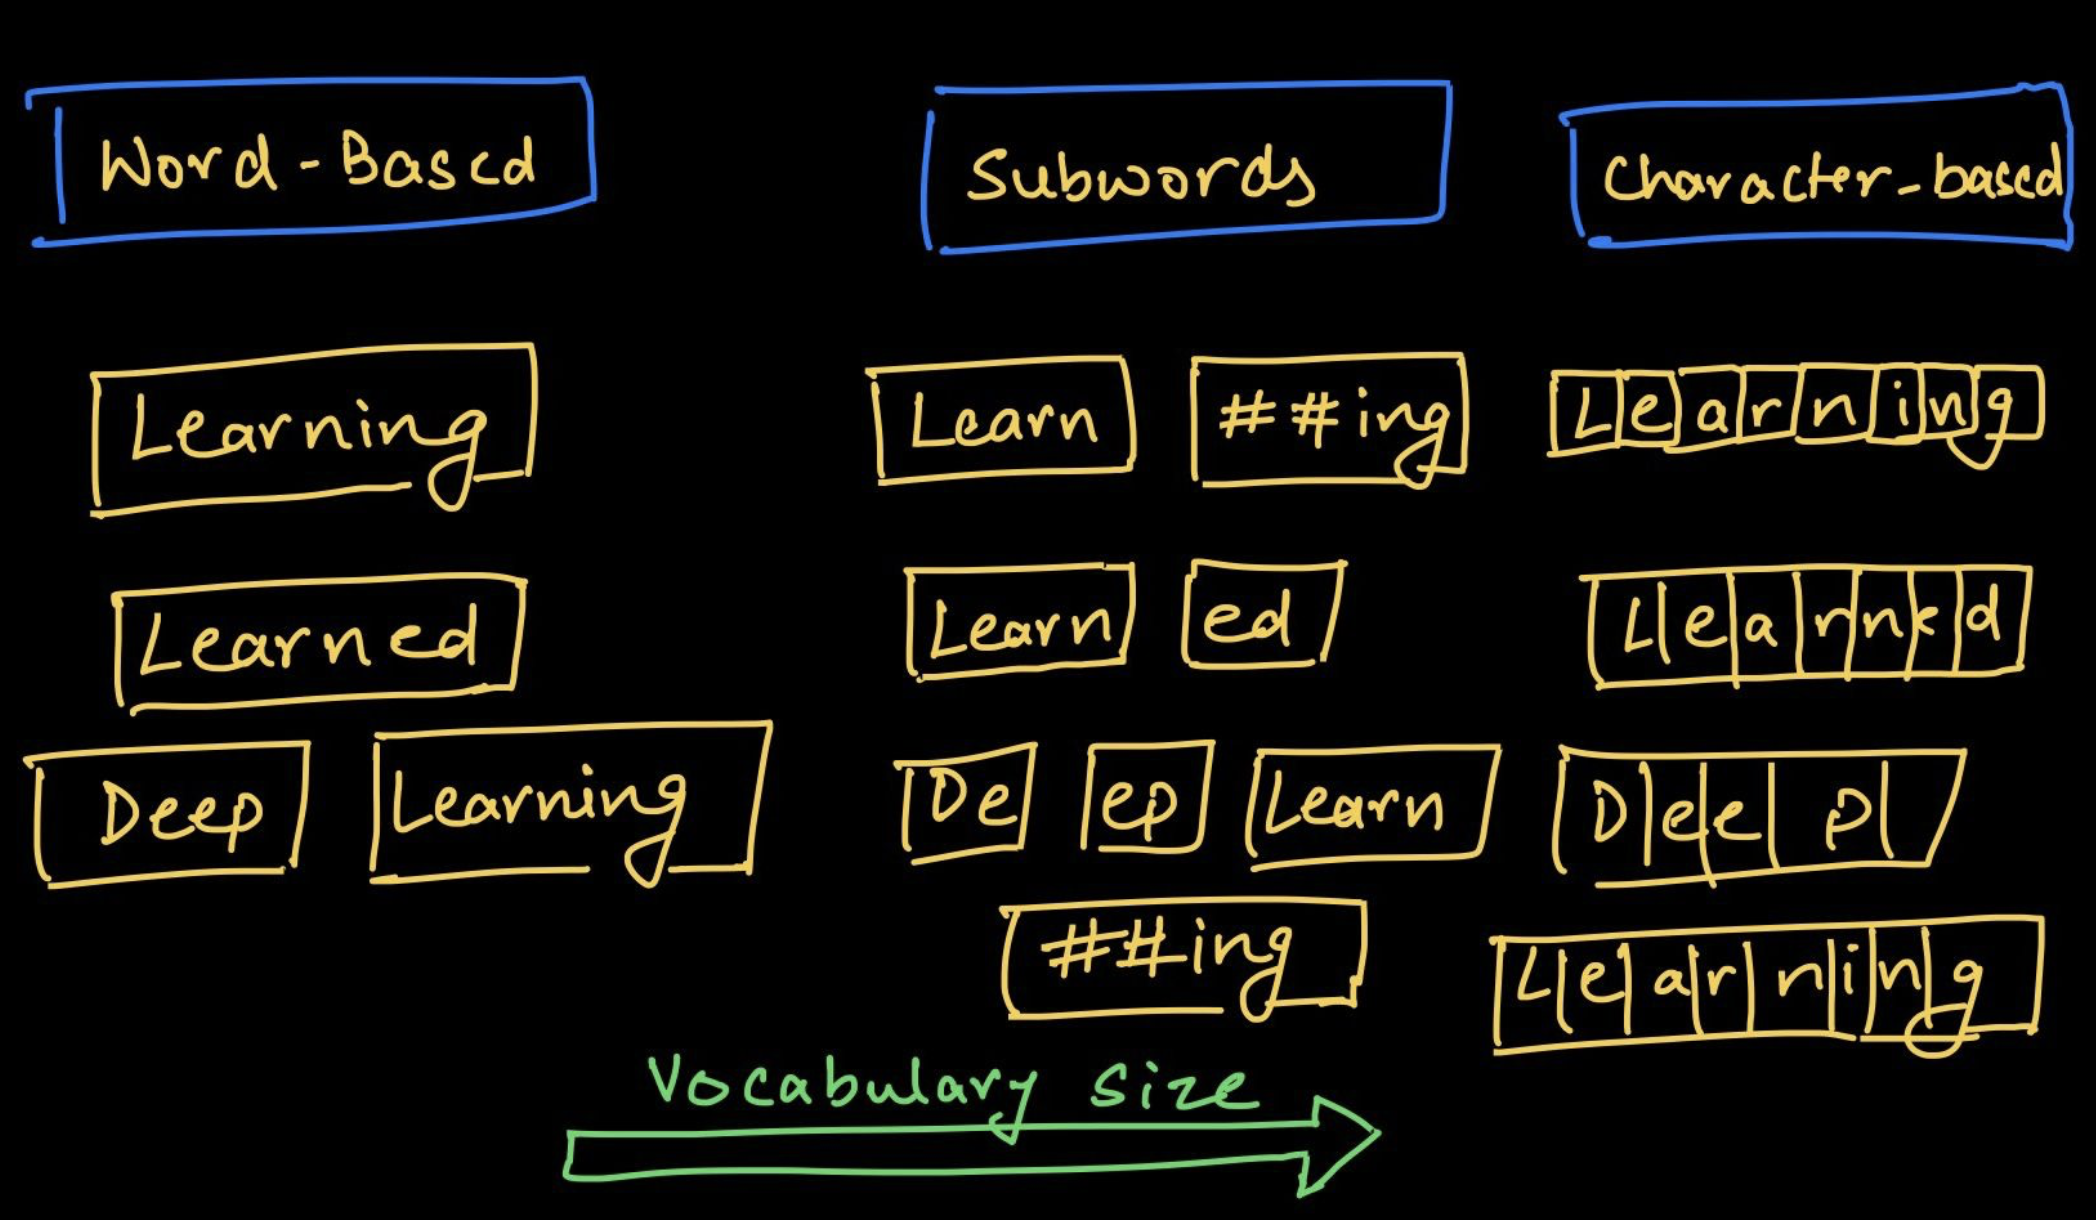
\includegraphics[scale=0.34]{tipo-tokenizador.png} 
		
		{\scriptsize Tomado de \url{https://www.freecodecamp.org/news/evolution-of-tokenization/}}
		
		\ifbool{false}
		{
			
			-> Por palabras
			
			Este método divide el texto en palabras individuales. Es el enfoque más común y es particularmente efectivo para idiomas con límites de palabras claros como el inglés.
			
			-> Por subpalabras 
			
			Aquí el texto está segmentado en caracteres individuales. Este método es beneficioso para idiomas que carecen de límites claros para las palabras o para tareas que requieren un análisis granular, como la corrección ortográfica.
			
			-> Subpalabras 
			
			Logra un equilibrio entre la tokenización de palabras y caracteres, divide el texto en unidades que pueden ser más grandes que un solo carácter pero más pequeñas que una palabra completa. Por ejemplo, los "Chatbots" podrían tokenizarse en "Chat" y "bots". Este enfoque es especialmente útil para lenguajes que forman significado combinando unidades más pequeñas o cuando se trata de palabras fuera de vocabulario en tareas de PNL.
		}
		
	\end{frame}
	
	%------------------------------------------------
	% Pos-tagged
	
	\begin{frame}
		
		\frametitle{Partes del discurso (tagged)}
		
		\begin{alertblock}{} 
			Objetivo: Identificar la parte de la oración de cada token, o sea, otorgar etiquetas.
		\end{alertblock}
		
		\vspace{1\baselineskip}
		\centering	
		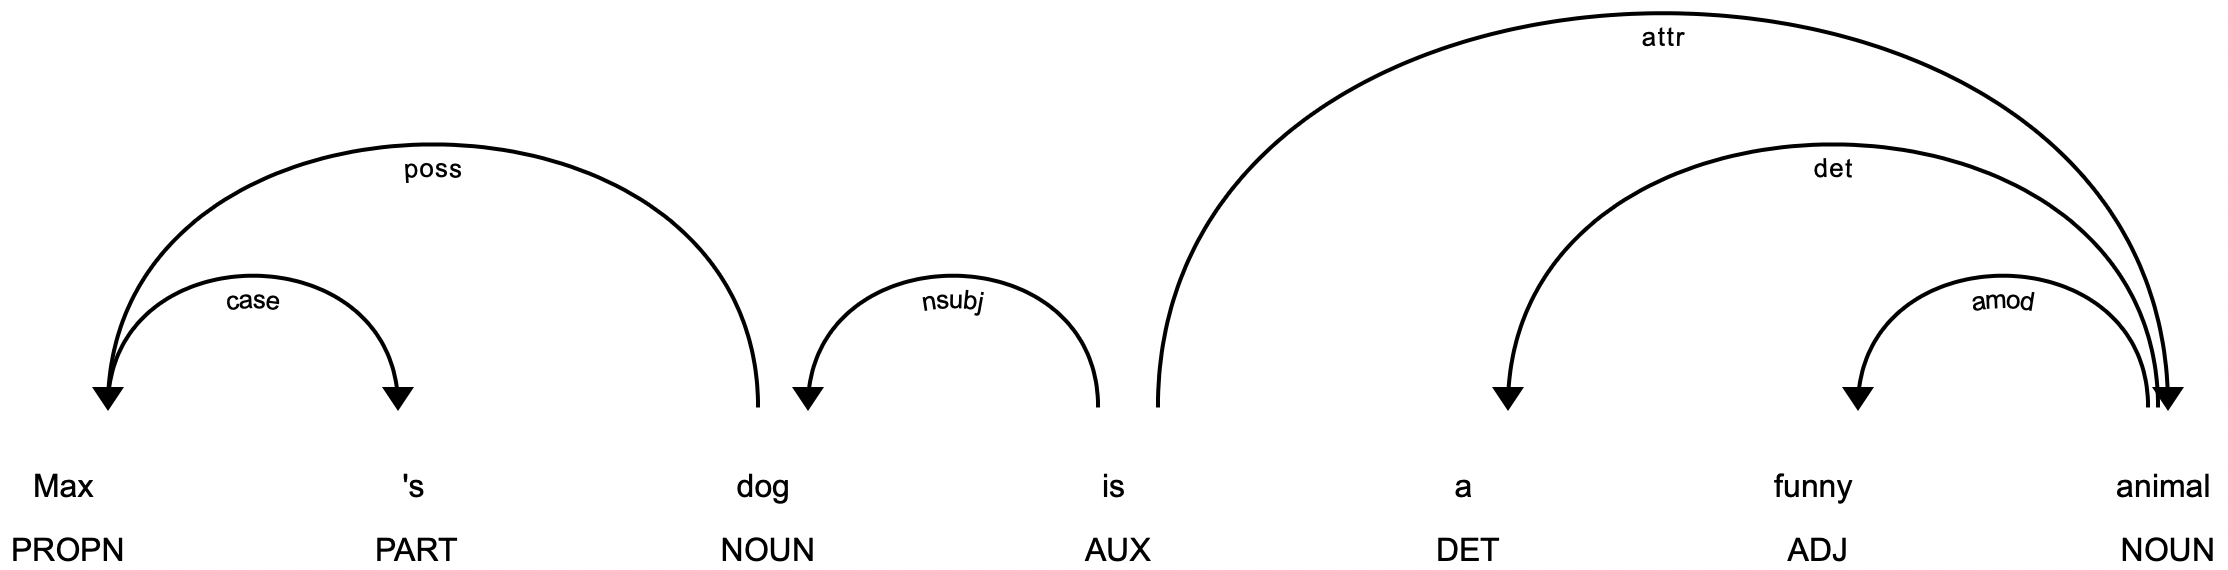
\includegraphics[scale=0.38]{pos-tagged.png} 
		
		\vspace{3\baselineskip}
		\pause
		\textcolor{purple}{¿Cómo nombrar cada token identificado?}
		
		
	\end{frame}
	
	%------------------------------------------------
	% Cadenas de Markov
	
	\begin{frame}
		
		\frametitle{Cadenas de Márkov} 
		
		\begin{block}{Markov Chains}
			Proceso estocástico discreto en el que la probabilidad de ocurrencia de un evento depende solamente del evento inmediatamente anterior, cumpliéndose que 
			$$P(q_i = a | q_0, \cdots, q_{i-1}) = P(q_i = a | q_{i-1})$$
			La relación anterior se considera como ``propiedad de Márkov''.
		\end{block}
		
		\pause 
		\noindent\begin{minipage}{.4\textwidth}
			\centering	
			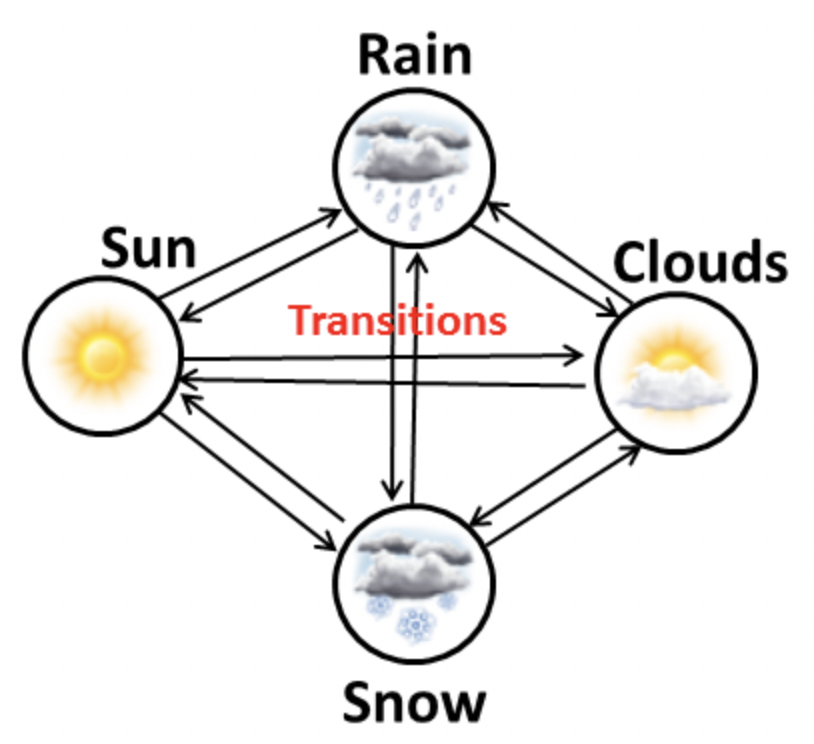
\includegraphics[scale=0.38]{cadena_markov.png} 
		\end{minipage}%
		\begin{minipage}{.6\textwidth}
			\vspace{2\baselineskip}
			
			Ejemplo para la predicción del tiempo 
			
			{\scriptsize Tomado de \url{https://espanol.libretexts.org/Biologia/Biolog\%C3\%ADa\_Computacional/Libro\%3A\_Biolog\%C3\%ADa\_Computacional\_-\_Genomas\%2C\_Redes\_y\_Evolución\_\%28Kellis\_et\_al.\%29/07\%3A\_Modelos\_ocultos\_de\_Markov\_I/7.03\%3A\_Cadenas\_de\_Markov\_y\_HMMS\_-\_Del\_ejemplo\_a\_la\_formalización}}
		\end{minipage}
		
	\end{frame}
	
	%------------------------------------------------
	% Modelo Oculto de Markov
	
	\begin{frame}
		
		\frametitle{Modelo Oculto de Markov}
		
		\begin{block}{Hidden Markov Model (HMM)}
			Modelo estadístico en el que se asume que el sistema a modelar es un proceso de Márkov con parámetros desconocidos. El objetivo es determinar las variables desconocidas u ocultas de la cadena a partir de los parámetros observables. 
		\end{block}
		
		\pause
		\noindent\begin{minipage}{.4\textwidth}
			\centering	
			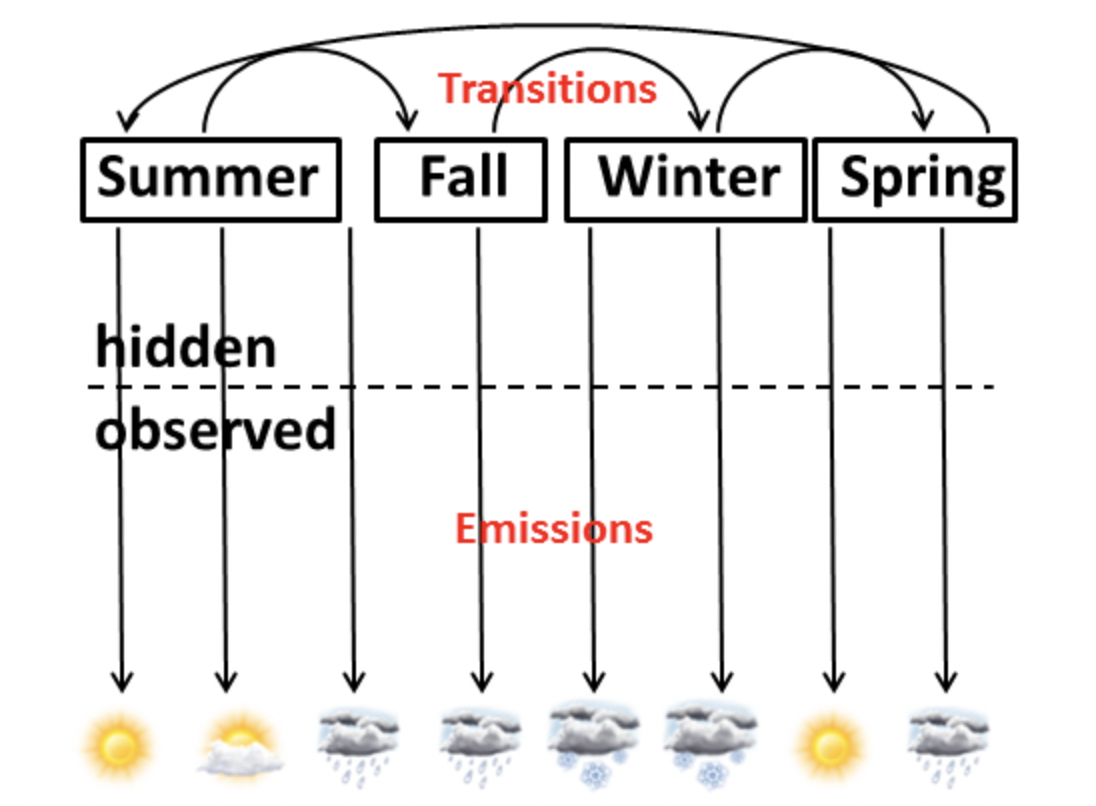
\includegraphics[scale=0.38]{cadena-oculta-markov.png} 
		\end{minipage}%
		\begin{minipage}{.55\textwidth}
			
			\begin{adjustwidth}{1.5cm}{} 
				
				Ejemplo para la predicción del tiempo 
				
				\pause
				\vspace{2\baselineskip}
				En NLP, las variables observadas son los tokens y las variables ocultas representan las etiquetas.
			\end{adjustwidth}
		\end{minipage}
		
	\end{frame}
	
	%------------------------------------------------
	% Reconocimiento de Entidades Nombradas
	
	\begin{frame}
		
		\frametitle{Reconocimiento de Entidades Nombradas (NER)}
		
		\begin{alertblock}{} 
			Objetivo: Identificar los objetos del mundo real.
		\end{alertblock}
		
		\pause
		\vspace{1\baselineskip}
		\begin{centering}
			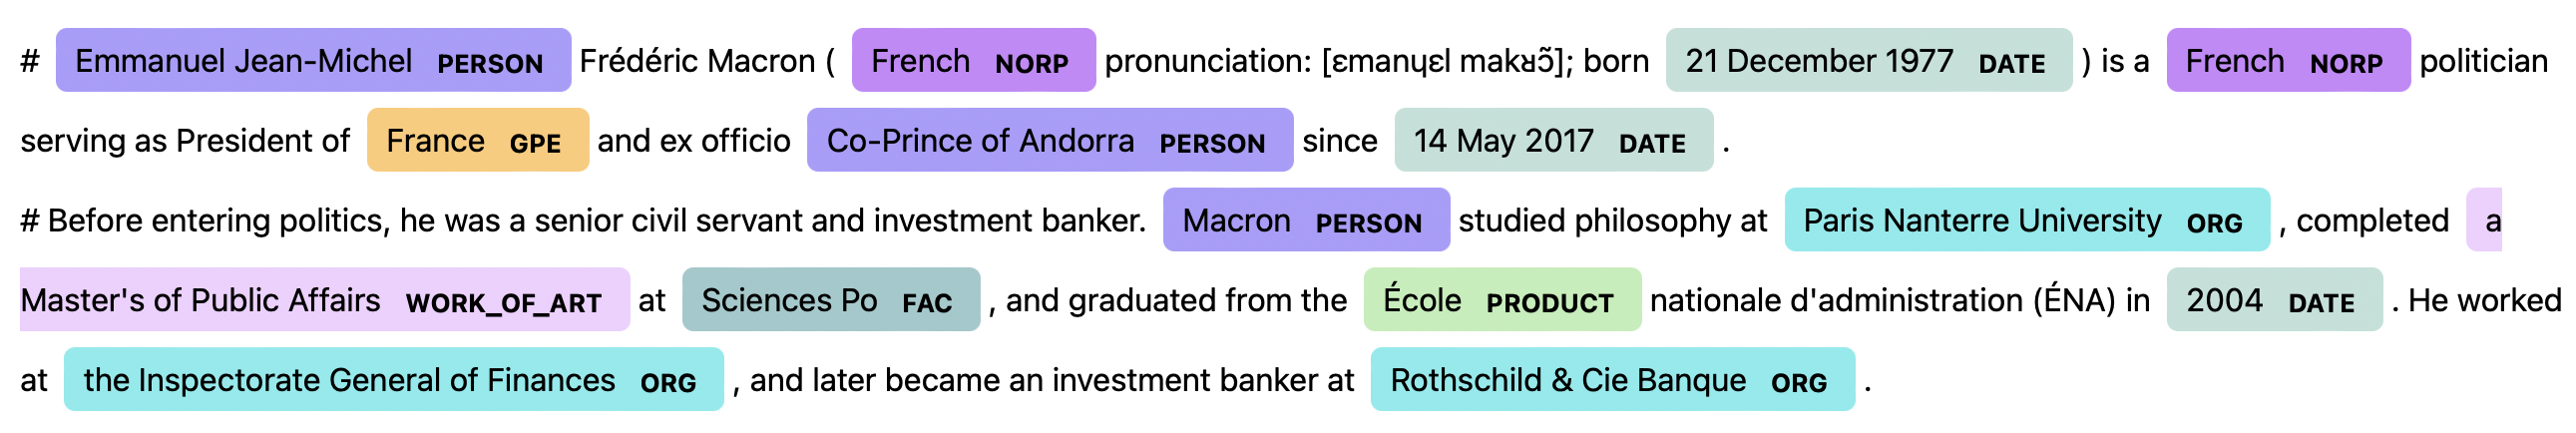
\includegraphics[scale=0.34]{ner.png}
		\end{centering}
		
		\vspace{1\baselineskip}
		
		\only<2>{\textcolor{purple}{¿Pero cómo?}}
		
		\only<3>{
			Posibles acercamientos: 
			\begin{itemize}
				\item Gacetas
				\item Modelo de Campos Aleatorios Condicionales (CRF, Conditional Random Fields)
				\begin{itemize}
					\item Caso general de HMM
					\item Usado para la predicción de estructuras en el texto
				\end{itemize}
			\end{itemize}
			
		}
		
	\end{frame}
	
	%------------------------------------------------
	% Tokenización y Segmentación
	
	\begin{frame}
		
		\frametitle{Del pre-procesamiento al procesamiento}
		
		% Explicación breve de cada una 
		
		\centering
		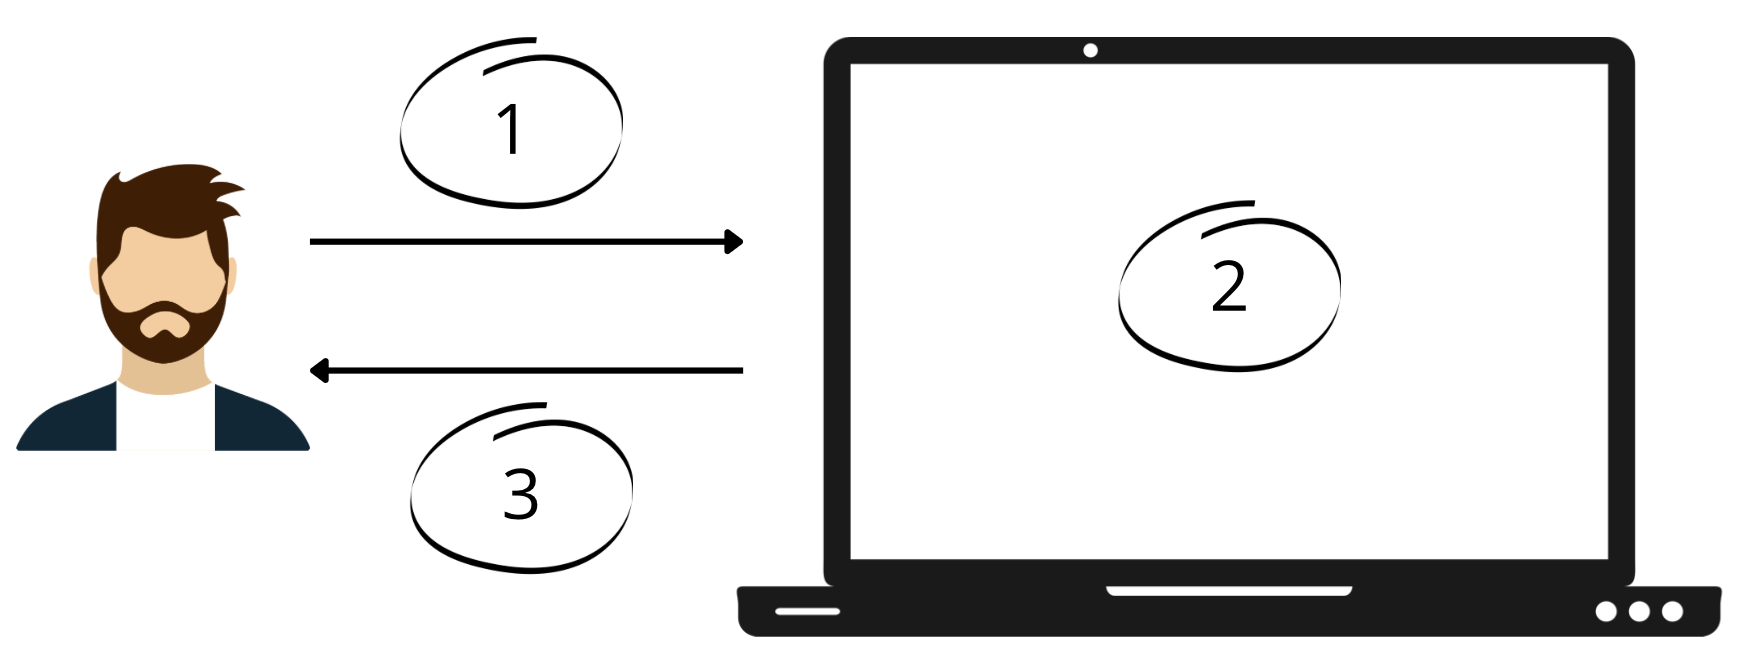
\includegraphics[scale=0.32]{motivacion.png} 
		
		\pause
		\begin{alertblock}{} 
			Un corpus es una colección de documentos.
		\end{alertblock}
		
		\vspace{2\baselineskip}
		\pause
		\textcolor{purple}{¿Cómo se representa computacionalmente un documento?}
		
	\end{frame}
	
	%------------------------------------------------
	% Representación de los documentos
	
	\begin{frame}
		
		\frametitle{Representación de los documentos}
		
		\begin{itemize}
			\item Bolsa de palabras (BoW, Bag of Word)
			
			\begin{itemize}
				\item Cada palabra del texto se considera una característica y la cantidad de veces que aparece una palabra en particular en el texto (\textbf{frecuencia}) se utiliza para representar la importancia de esa palabra en el texto.
			\end{itemize}
			
		\end{itemize}
		
		\pause
		\vspace{2\baselineskip}
		
		\centering
		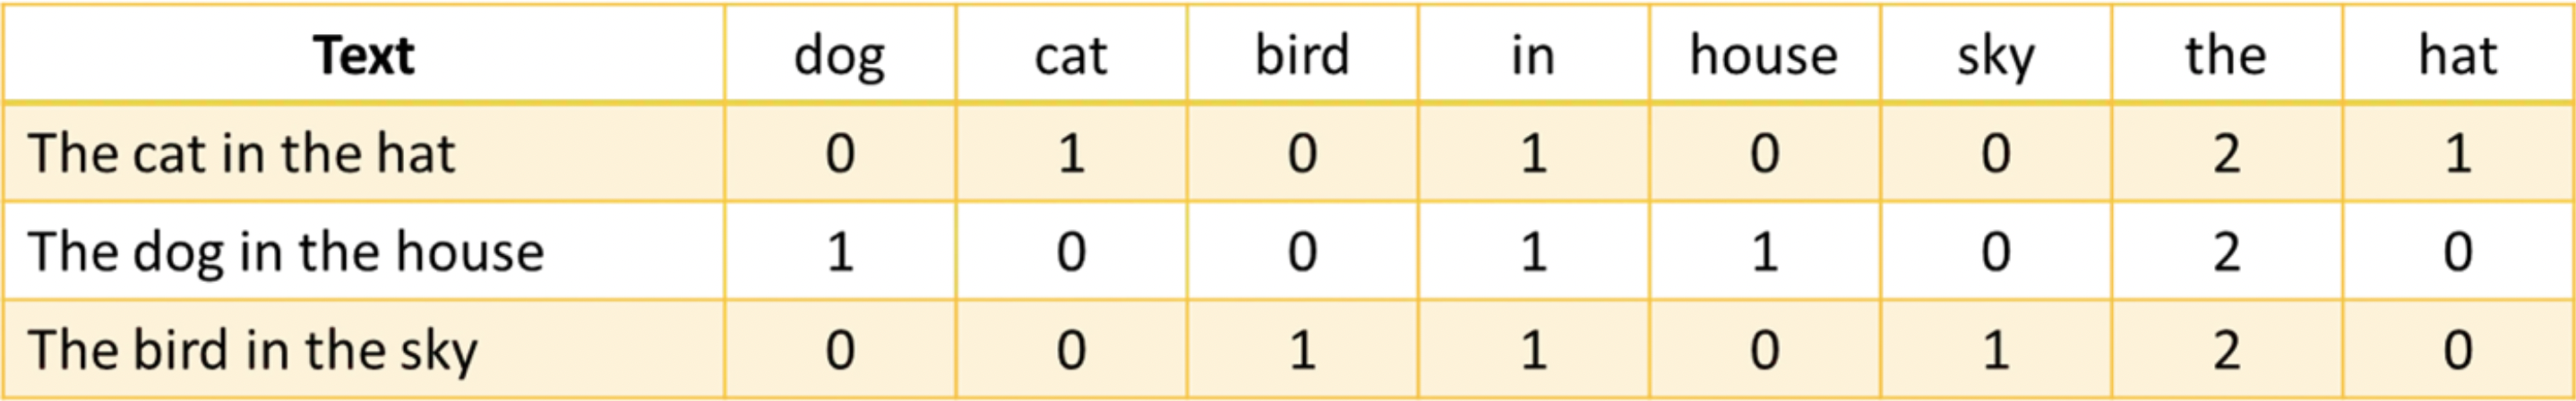
\includegraphics[scale=0.3]{bow.png}
		
		{\scriptsize Tomado de \url{https://deysusovan93.medium.com/from-traditional-to-modern-a-comprehensive-guide-to-text-representation-techniques-in-nlp-369946f67497}}
		
	\end{frame}
	
	%------------------------------------------------
	% Representación de los documentos
	
	\begin{frame}
		
		\frametitle{Representación de los documentos}
		
		\begin{itemize}
			\item $N$-grama
			
			\begin{itemize}
				\item Técnica que implica dividir el texto en secuencias contiguas de $N$ palabras
				
				\pause
				\item Ejemplo ``The dog in the house''
				\begin{itemize}
					\item \textbf{Uni-grama}: ``The'', ``dog'', ``in'', ``the'', ``house''
					\item \textbf{Bi-grama}: ``The dog'', ``dog in'', ``in the'', ``the house''
					\item \textbf{Tri-grama}: ``The dog in'', ``dog in the'', ``in the house''
				\end{itemize}
				
			\end{itemize}
			
		\end{itemize}
		
		% hablar de las ventanas
		
	\end{frame}
	
	%------------------------------------------------
	% Representación de los documentos
	
	\begin{frame}
		
		\frametitle{Representación de los documentos}
		
		\begin{itemize}
			\item TF-IDF
			
				\begin{itemize}
				\item Técnica que implica dividir el texto en secuencias contiguas de $N$ palabras, otorgando peso
				$$w_{i,j} = tf_{i, j} \times idf_i =(\alpha + (1 - \alpha) \frac{freq_{i,j}}{max_l freq_{l, j}}) \times \log(\frac{N}{n_i}) $$
				
				\pause
				\item Es mejor que BoW porque destaca la importancia de las palabras en cada documento	
			\end{itemize}
			
		\end{itemize}
		
		\pause
		\vspace{2\baselineskip}
		
		\centering
		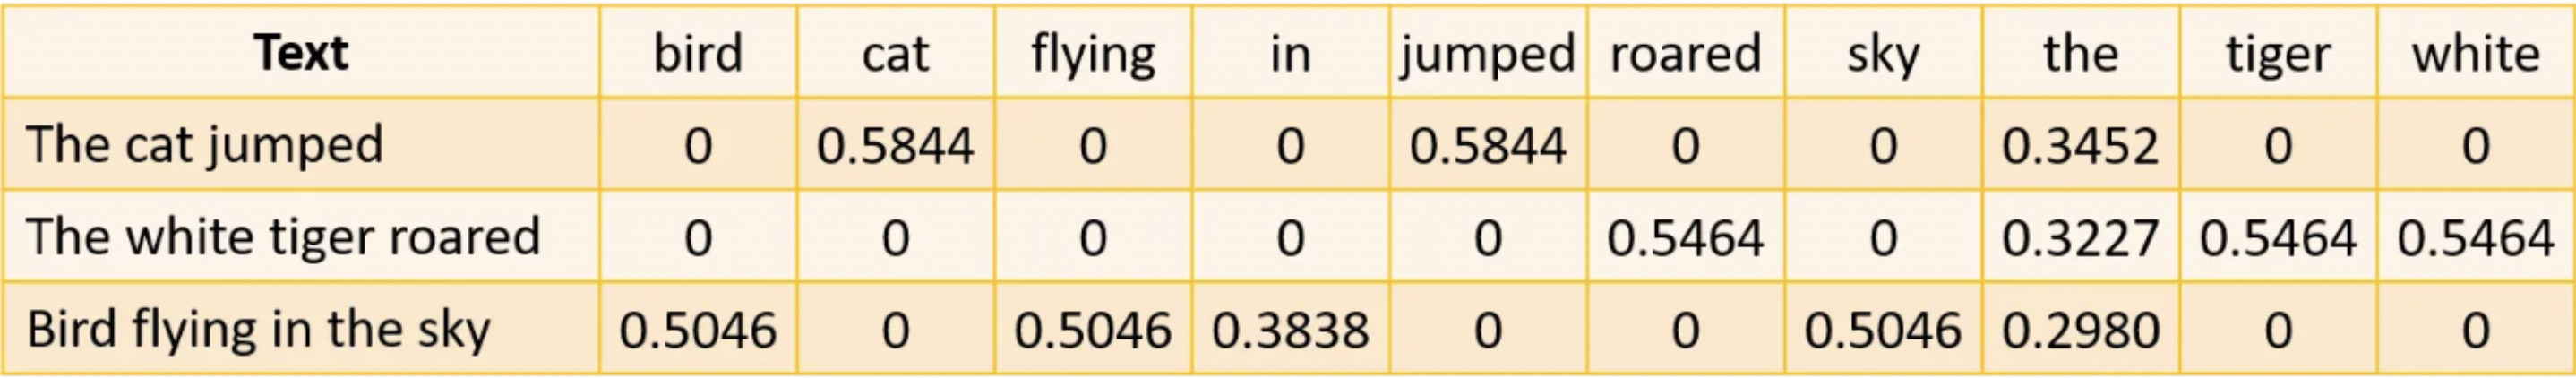
\includegraphics[scale=0.3]{tf-idf.png}
		
		{\scriptsize Tomado de \url{https://deysusovan93.medium.com/from-traditional-to-modern-a-comprehensive-guide-to-text-representation-techniques-in-nlp-369946f67497}}
		
	\end{frame}
	
	%------------------------------------------------
	% Representación de los documentos
	
	\begin{frame}
		
		\frametitle{Representación de los documentos}
		
		\begin{itemize}
			\item Word embedding
			
			\begin{itemize}
				\item Representa cada palabra como un vector denso de números reales, de modo que las palabras similares o estrechamente relacionadas están más cerca entre sí en el espacio vectorial.
				
			\end{itemize}
			
		\end{itemize}
		
		\pause
		
		\centering
		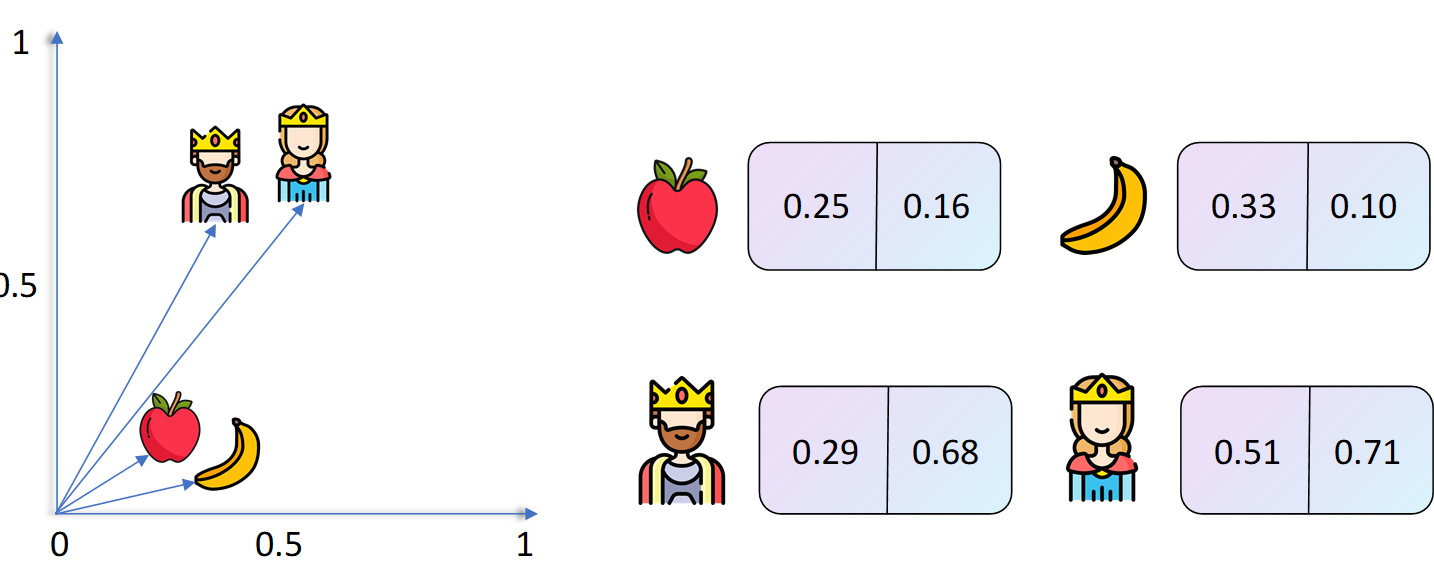
\includegraphics[scale=0.25]{word-embedding.png}
		
		{\scriptsize Tomado de \url{https://towardsdatascience.com/deep-learning-for-nlp-word-embeddings-4f5c90bcdab5}}
		
	\end{frame}
	
	%------------------------------------------------
	% Reducción del vocabulario
	
	\begin{frame}
		
		\frametitle{Reducción del vocabulario}
		
		Palabras como \textbf{democracy}, \textbf{democratic} o \textbf{democratization} hacen referencia al concepto de \textbf{democracy} y representan tokens.
		
		
		\vspace{2\baselineskip}
		\pause
		\textcolor{purple}{¿Cómo se pueden sustituir las palabras ``parecidas'' o ``similares'' por otra que las identifique de igual manera?}
		
		\pause
		\vspace{1\baselineskip}
		Ejemplo: the boy's cars are different colors $\Rightarrow$ the boy car be differ color
		
		\centering
		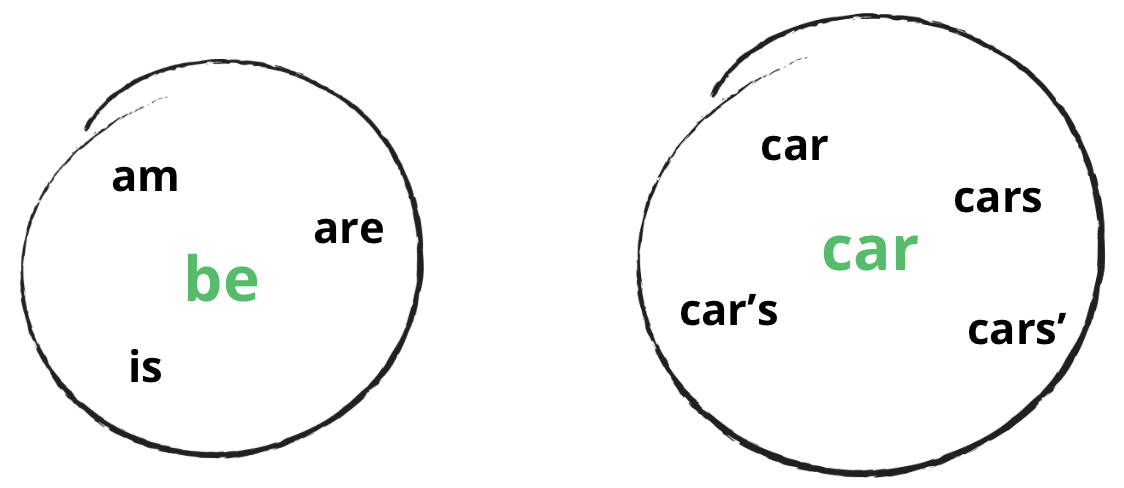
\includegraphics[scale=0.45]{lema.png}
		
	\end{frame}
	
	%------------------------------------------------
	% Reducción del vocabulario. Lematización
	
	\begin{frame}
		
		\frametitle{Reducción del vocabulario}
		
		\begin{itemize}
			\item Lematización
			
			\begin{itemize}
				\item Proceso en el cual haciendo uso correcto del vocabulario y análisis morfológico de las palabras, devolver la forma base de la palabra, lo que se conoce como lema.
				
				\item El lema es una palabra real.
				
				\item Considera el contexto.
				
				\item Computacionalmente costoso.
				
				\item Utiliza reglas lingüísticas para determinar el lema durante el proceso de tokenización.
				
				\pause
				\item Ejemplo: 
				\begin{itemize}
					\item running $\Rightarrow$ run
					\item better $\Rightarrow$ good
				\end{itemize}
				
			\end{itemize}
		
		\end{itemize}
		
	\end{frame}
	
	%------------------------------------------------
	% Reducción del vocabulario
	
	\begin{frame}
		
		\frametitle{Reducción del vocabulario}
		
		\begin{itemize}
			\item Stemming
			
			\begin{itemize}
				\item Proceso heurístico crudo que ``corta'' los extremos de las palabras.
				
				\item A menudo conduce a significados y ortografías incorrectos.
				
				\item Muy utilizado para trabajar con conjuntos de datos grandes donde el rendimiento es un problema.
				
				\item El algoritmo más utilizado en Inglés es el algoritmo de Porter [Porter, Martin F., An algorithm for suffix stripping, 1980, Program 14 (3): 130-137], el cual consiste en 5 fases secuenciales de reducción de las palabras. Por ejemplo, la primera frase se describe como: 
				
				\begin{centering}
					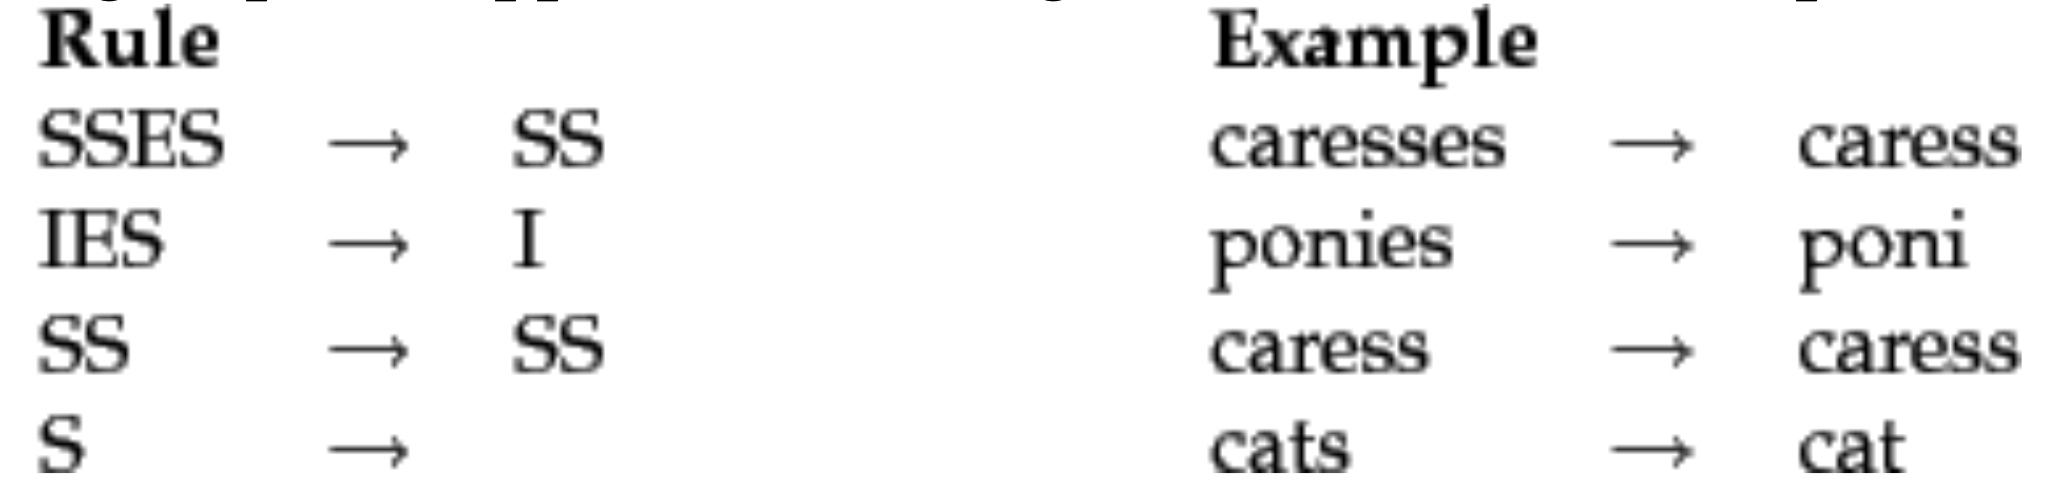
\includegraphics[scale=0.25]{porter.png}
				\end{centering}
				
				\pause
				\item Ejemplo:
				
				\begin{centering}
					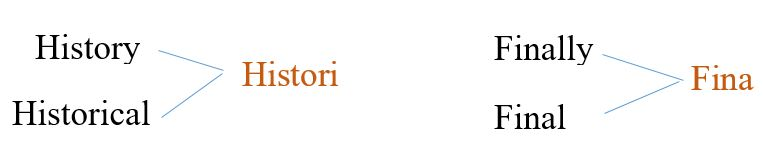
\includegraphics[scale=0.7]{stemming.jpg}
				\end{centering}
				
			\end{itemize}
			
		\end{itemize}
		
	\end{frame}
	
	%------------------------------------------------
	% Tipos de ambigüedad
	
	\begin{frame}
		
		\frametitle{Tipos de ambigüedad}
		
		\begin{itemize}
			
			\item Por polisemia
			
			\only<2->{
				\begin{forest}
					for tree={grow'=south, anchor=north}
					[ 
						Esto pinta muy bien, 
						[Un objeto sirve para pintar]
						[La situación tiene buen aspecto]
					]
				\end{forest}
			}
			
			
			\item Por impresición gramatical
			
			\only<3->{
				\begin{forest}
					for tree={grow'=south, anchor=north}
					[ 
						{Cuando el ladrillo chocó con la pared, se rompió}, 
						[El ladrillo se rompió al chocar la pared]
						[La pared se rompió al chocar el ladrillo contra ella]
					]
				\end{forest}
			}
			
			\item Por la sintaxis
			
			\only<4->{
				\begin{forest}
					for tree={grow'=south, anchor=north}
					[ 
						Canto espléndido, 
						[Yo canto espléndidamente]
						[Canción espléndida]
					]
				\end{forest}
			}
						
		\end{itemize}
		
	\end{frame}
	
	%------------------------------------------------
	% Algoritmos para desambiguar
	
	\begin{frame}
		
		\frametitle{Algoritmos para desambiguar}
		
		\begin{itemize}
			\item Basados en conocimiento: 
			\begin{itemize}
				\item Uso de recursos como diccionarios y tesauros
			\end{itemize}
			
			\pause 
			\vspace{2\baselineskip}
			\item Basados en corpus
			\begin{itemize}
				\item Uso de técnicas estadísticas y de aprendizaje automático para inducir modelos del lenguaje natural a partir de grandes conjuntos de ejemplos textuales 
			\end{itemize}
		
		\end{itemize}
		
	\end{frame}
	
	%------------------------------------------------
	% Ejemplos de uso de NLP
	
	\begin{frame}[fragile]
		
		\frametitle{Ejemplos de uso de NLP}
		
		\begin{itemize}
			\item Predicción del texto
		\end{itemize}		
		
		\centering
		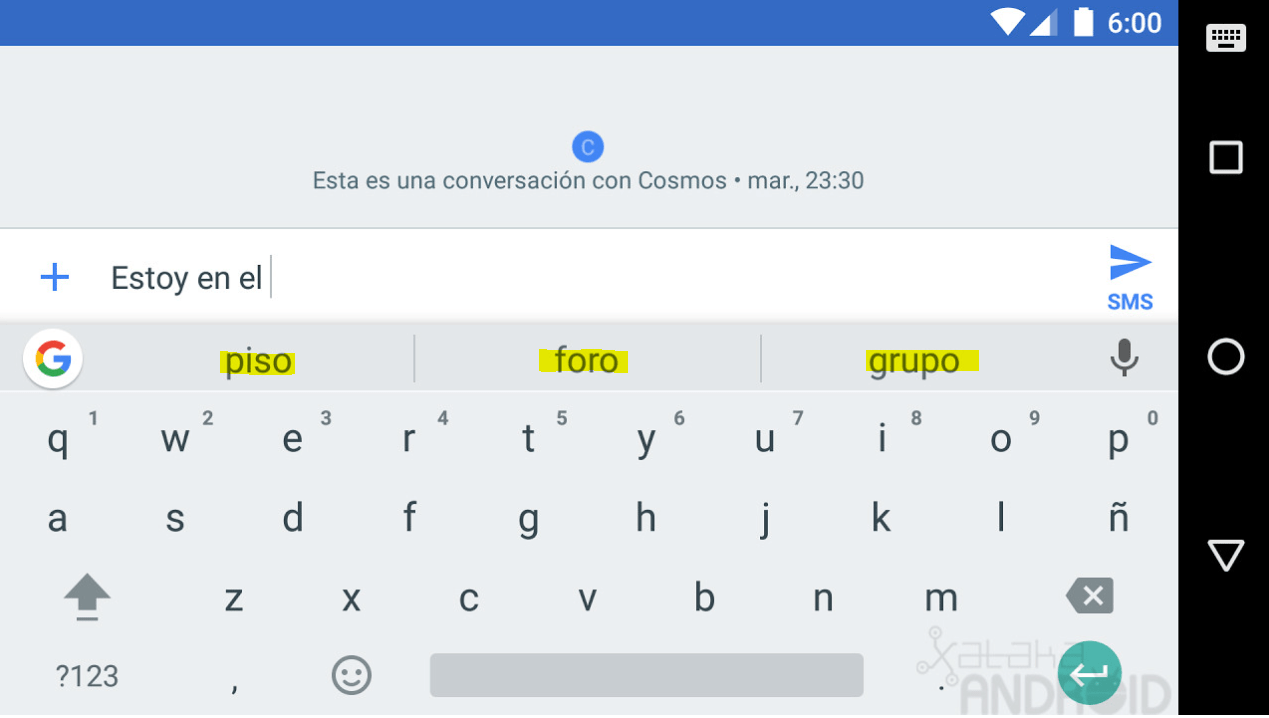
\includegraphics[scale=0.4]{teclado-predictivo-xataka-android.png}
		
		{\scriptsize Tomado de \url{https://www.plenainclusion.org/discapacidad-intelectual/recurso/teclado-predictivo/}}
		
	\end{frame}
	
	%------------------------------------------------
	% Ejemplos de uso de NLP
	
	\begin{frame}
		
		\frametitle{Ejemplos de uso de NLP}
		
		\begin{itemize}
			\item Extracción de variables latentes (LDA, Latent Dirichlet Alocation)
		\end{itemize}		
		
		\centering
		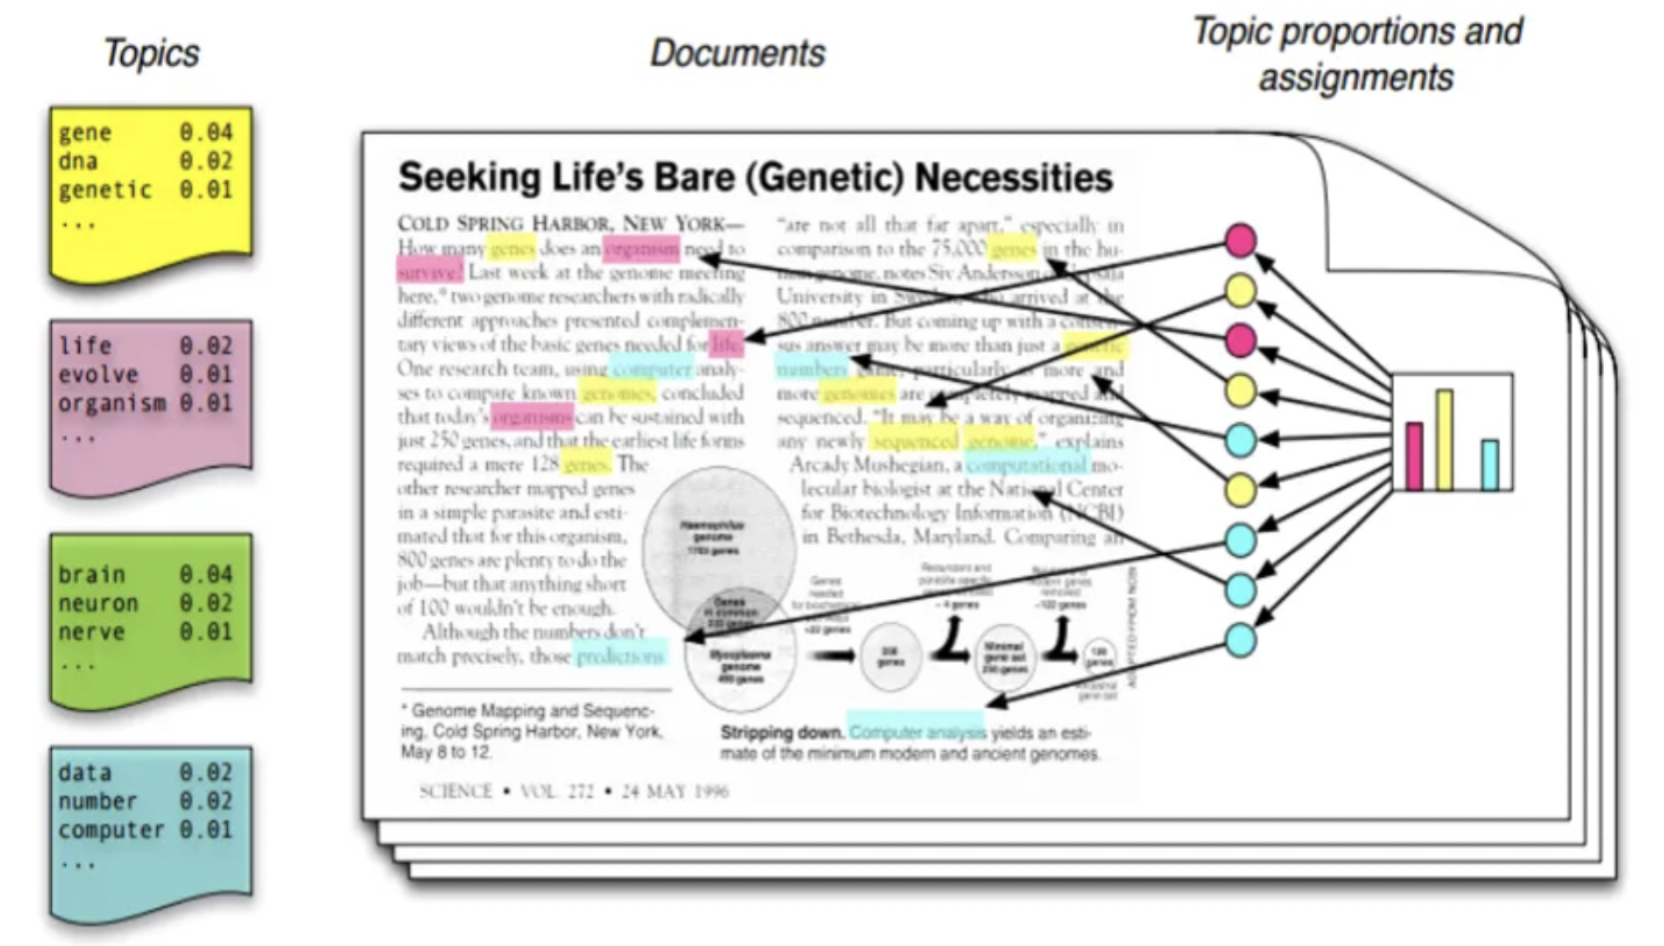
\includegraphics[scale=0.4]{lda.png}
		
		{\scriptsize Tomado de \url{https://towardsdatascience.com/the-complete-guide-for-topics-extraction-in-python-a6aaa6cedbbc}}
		
	\end{frame}
	
	%------------------------------------------------
	% Dudas
	
	\begin{frame}
		
		\frametitle{Dudas, preguntas, sugerencias ...}
		
		\begin{figure}[h]
			\centering
			
\includegraphics[scale=0.38]{duda.png}
		\end{figure}
		
	\end{frame}
	
	%------------------------------------------------
	% Bibliografía
	
	\begin{frame}
		
		\frametitle{Bibliografía}
		
		\begin{itemize}
			
			\item Srinivasa-Desikan, Bhargav, ``Natural Language Processing and Computational Linguistics: A Practical Guide to Text Analysis With Python, Gensim, spaCy, and Keras'', 2018			
			
			\item \url{https://nlp.stanford.edu/IR-book/html/htmledition/stemming-and-lemmatization-1.html}
			
			\item \url{https://spacy.io}
			
			\item \url{https://nlp.stanford.edu/IR-book/html/htmledition/stemming-and-lemmatization-1.html}
			
		\end{itemize}
		
	\end{frame}
	
	%------------------------------------------------
	% Fin
	
	\begin{frame}
		\titlepage
	\end{frame}
	
	
	
\end{document} 